\chapter[活的安全案例：发布与保证本体]{活的安全案例：\\发布与保证本体}

\begin{noteblock}
Semantica 绑定： 本章保存持续保证、发布绑定和人机决定边界；唯一机器语义是
\nolinkurl{semantica.chapter_packages.vol2.ch20}，主场景为
\nolinkurl{semantica.vol2.ch20.scenario.primary}。本体、CQ、查询、Shape、正反案例、工程规则、
legacy capstone 迁移证据、oracle、snapshot、PROV、receipt 与 release verdict
均在 Semantica。当前为 \nolinkurl{partial}、release \nolinkurl{blocked}；机器把候选算到可审查，
不能替有权人签字，也不能把被阻断的发布说成完成。
\end{noteblock}

\begin{center}
\vspace{0.2em}
\chapterartfade{%
\adjustbox{max size={0.88\linewidth}{0.27\textheight}}{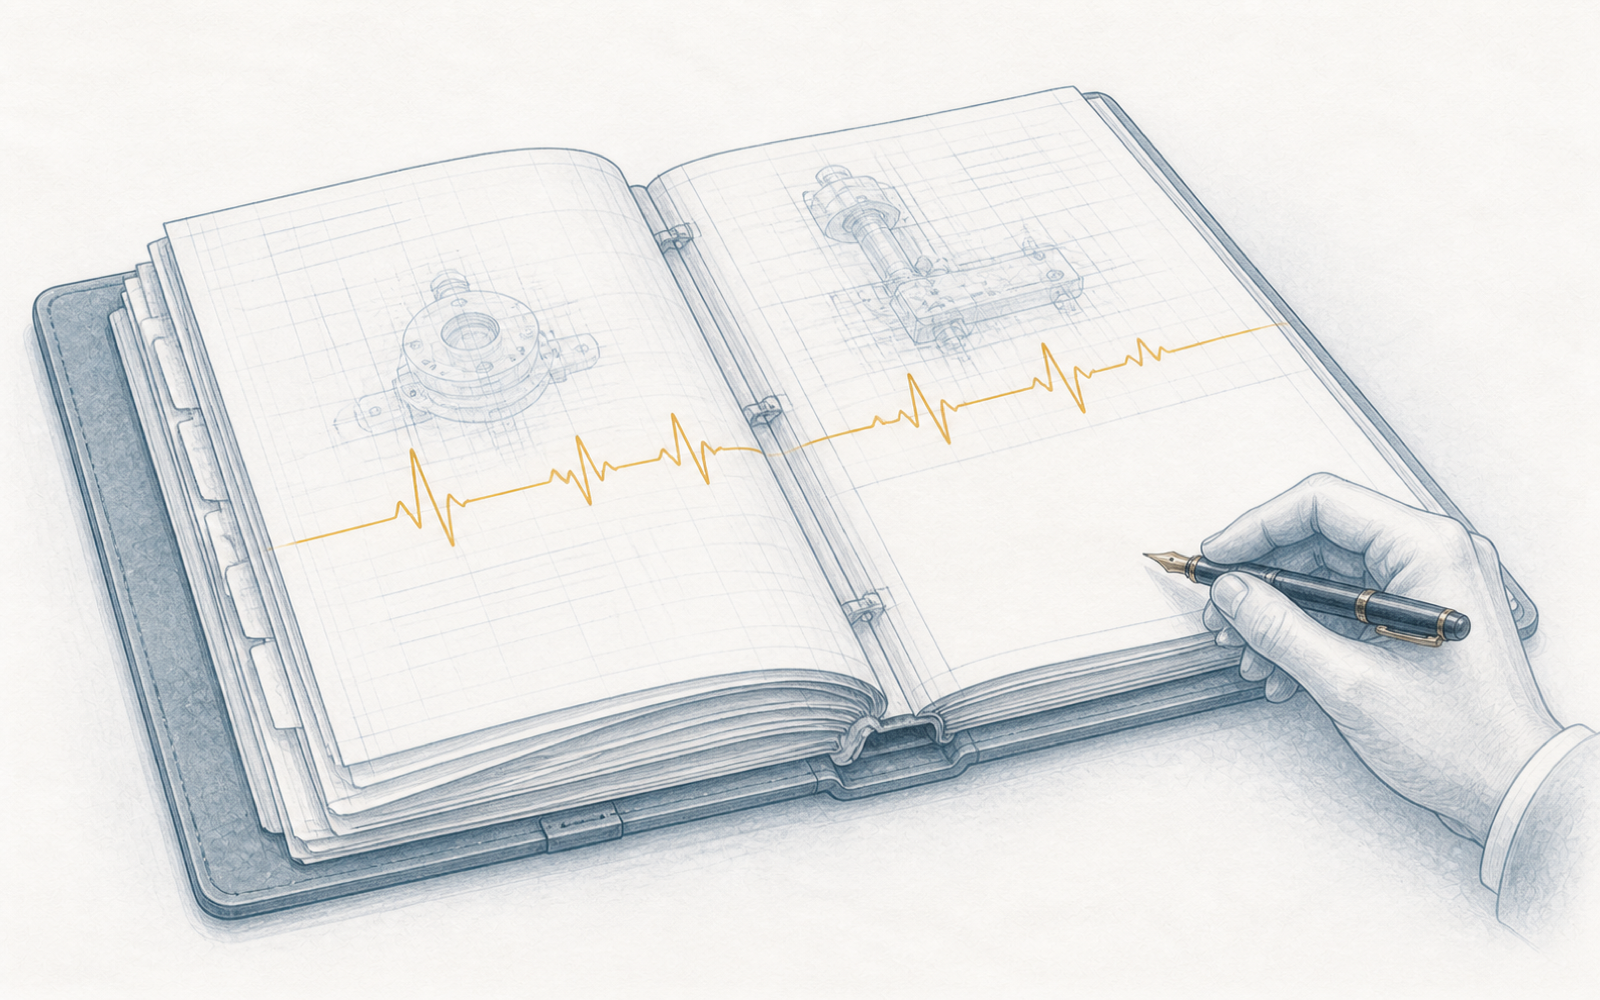
\includegraphics{figures-imagegen/art-ch20-v01.png}}%
}
\vspace{0.35em}
\end{center}

\begin{noteblock}
\textbf{【导读】}
试点走到最后一站，要换载体的轮到放行桌自己。本章先把前半部收口时冻结的三个
“纸面到不了的地方”翻译成机器必须能回答的问题；再用一个最小的发布保证本体，
把发布快照、证据包、主张—论证—证据三层、冲突、重开条件与授权决定一一变成对象；
然后让那个深夜的旧事故第二次发生——这一次在装包的当口就被拦下；让一场从天而降的
模型升级考验这套结构里什么会死、什么会活；最后陪 RC18 走完第一场“活的”放行评审，
把全书悬着的三个问题收回来。
读完本章，你应当能说出一份安全案例怎样才算活着——它靠什么自己对表、自己现身、
自己举手，又在哪一步必须把笔交还给人。
\end{noteblock}

\Needspace{6\baselineskip}
\section{十套语言，回到一张桌子}

试点进行到第十一个月，放行桌上最先消失的是推车。从设计到现场，每一环的证据不再
装箱运来，而是各自以对象的身份住在自己的世界里：担心与目标住在危害那边，需求与
派生理由住在追溯那边，数字带着来源住在测量那边，版本与变更住在变化那边，依赖与
共因住在依赖那边，批次与单件住在制造与现场那边。老何上个月刚用单件履历把一次
嫌疑圈定从两千一百台压到七百台以内；此刻他把那条批次—单件链的出口，接到了
放行桌上。全链证据都回得来了。问题只剩一个，也是当初冻结时的最后一个：
案例能不能活起来？

牵头收这一站的还是小蔡。一年前她还是那个把三百多份文件装进三个纸箱、以为“装订
好就齐了”的新人；如今九个本体的对齐合同上，一半有她的名字。试点作战室的墙上贴着
三句话，是她从那次收口评审抄回来的，也是前半部留下的总账：证据包没法自己
核对同一基线；变更影响靠人工圈定；安全案例是死文档，产品是活的。试点的最后一站，
就是把这三句话逐句销账。而放行这一站还有个别处没有的难处：前面九个本体在这张桌上
全要露面。RC17 当年写下的三条重开条件，先后响了两条——升版获准落地，决定窗口
到期。于是有了新一轮候选 RC18：H3.2 硬件、转为正式版的 SW1.8.4、经差异分析确认
沿用的 C41，D7 与 V12 依旧。它的放行，就是这场试点的毕业考试。

动手之前，先冒出来一个所有人都动过的念头。这次把它说出口的是小唐：“咱们手里
已经九套词汇了，加上这套是十套。放行桌上哪一套都躲不开——那不如趁收尾把十个本体
合成一张总图，以后维护一处、查询一处，一劳永逸。”

这个提议一点都不外行。把分散的模型统一成一个大模型，是数据库年代真实成功过的
路线；十套词汇十套账，任谁看着都觉得冗余。小蔡没有争论，她请助手做了一下午试验：
先挑两家试着并——把测量那边的“受测对象”与制造那边的“物理单件”合成一个类。
下午还没过完，试验自己停了。两家对“还是不是同一个”的判据本来就不同：一边按
配置与构建认同一，一边按序列号与履历认同一；硬并成一个类，等于逼着两家共用一套
身份判据——那正是当年花了一整章才拆开的东西。更要命的是看守：每个本体都有自己的
看守人、自己的完备性声明、自己的重开纪律，一张大图归谁看守？改一条边，十个领域
一起震动——制造那边想给单件补一条报废去向的边，得先问过测量、变更、依赖各家
答不答应——结局不是一劳永逸，是谁也不敢动。

那就换个方向偷懒：十个本体不动，放行桌自己再建一套“什么都说一遍”的超级本体，
把各家内容复述进来。这条路更隐蔽也更糟——复述的那一刻就开始漂移，从此世上有
两份真相，每次不一致都要开会裁决谁算数。同名异义的老病，换了载体又要复发。

小唐听完试验汇报，自己把提议收了回去。陈工只补了一句裁决：“十个院子十把锁。
这张桌上，只摆各家愿意交出来的钥匙牌。”

两条路都堵住，放行本体该长什么样才显出来。放行桌需要知道的其实很薄：每份证据
是谁、绑定在哪个快照上、作证到哪里、此刻什么状态、归谁看守——至于它内部更深的
结构，留在自家本体里，经显式对齐合同按需去查。\textbf{放行需要的不是一张吞下一切的大图，而是每个本体守好自家边界之后，愿意向桌面交出的那层薄接口。}十个本体
还是十个，桌面上多出来的只是一层。

薄归薄，这层接口要接住的却是三句重话。把墙上的账翻译成机器必须能回答的问题，
就是这个本体的验收边界。其一，任何时刻问“这个证据包的成员是否全部绑定同一个
发布快照”，机器要能直接回答，并指认出不合群的那一份——不再依赖谁深夜逐行抄表。
其二，任何一处获准的变更落地之后，问“案例里哪些主张、论证与证据关系因此过期、
哪些决定需要重开”，答案要从结构里查出来，不再出自某个人的私人记忆。其三，
任何时刻问“这份案例现在的状态”——哪些在案、哪些过期、哪些未知、哪些缺口、
谁看守、什么条件下重开——案例要能自己举手，而不是躺在库里等人想起。

三个问题都要机器作答，案例就不能再是一摞文档。它得变成东西——变成什么样的东西？

\Needspace{6\baselineskip}
\section{把案例变成对象：最小发布保证本体}

第一步还是老老实实把话说白。

发布快照，是那句大主张的主语：一组配置的共同身份。第 1 章补主语、补配置补出来的
东西，在这里第一次成为可以被指着说的对象，而不是封面上的一行字。证据包，是一次
放行所引用证据的显式集合。关键动作有两个：包自己声明“我属于哪个快照”，每个成员
各自声明“我绑定在哪个快照”——两处声明必须相等。“同一基线”从此不是核对出来的
结论，而是结构里一条可查的边。

这段记法在说什么：下面立出 RC18 这个快照和它的证据包。注意三处细节——五项配置
\Needspace{8\baselineskip}
各是对象；包上那行“清单已记全”；以及成员自带的两条边。

\nopagebreak[4]
\begin{codebox}
\begin{Verbatim}[fontsize=\small,breaklines=true,breakanywhere=true,breaksymbolleft={},breaksymbolright={}]
# 发布快照与证据包（示意记法）
rel:RC18 a rel:ReleaseSnapshot ;
    rel:configItem rel:HW_H32 , rel:SW_184 ,
                   rel:CAL_C41 , rel:DRV_D7 , rel:BASE_V12 .
rel:PKG_RC18 a rel:EvidencePackage ;
    rel:declaredSnapshot rel:RC18 ;          # 包声明自己属于谁
    rel:hasMember        rel:SWRegReport_r11 ;
    rel:memberListClosed true .              # 清单已记全，缺席可判
rel:SWRegReport_r11
    rel:boundTo    rel:RC18 ;                # 成员自带绑定
    rel:producedBy rel:SWRegRun_r11 .        # 事实出自受控活动
\end{Verbatim}
\end{codebox}

“清单已记全”那一行最容易被看轻，它是机器有资格喊“缺”的前提：只有在被告知
成员清单已经封口之后，论证里引用了、包里却没有的那张卡，才成立为缺口，而不是
永远的沉默。最后一行也不是装饰：每份证据必须指回产出它的受控活动——本体负责
说清这份证据是什么，而它作证的内容真不真，只能由台架、产线与试验场的活动记录
负责。语义与事实，从进门第一行就分账。

第二步，把当年那场“写在纸上的辩护”逐层对象化。主张是对象，论证是对象，证据是
对象；论证引用证据的每一次引用是一条边；而方工说过“论证是唯一不能由单个专业
交出的东西”，那句“为何这些证据合起来够了”的理由，现在也写成对象的属性，
不再只活在会议室的空气里。

这段记法在说什么：三层结构挂好之后，把当年写在纸上的重开条件也变成对象——
\Needspace{8\baselineskip}
注意它的看守人是一个角色，不是一个人名。

\nopagebreak[4]
\begin{codebox}
\begin{Verbatim}[fontsize=\small,breaklines=true,breakanywhere=true,breaksymbolleft={},breaksymbolright={}]
# 主张—论证—证据三层，外加重开条件（示意记法）
rel:Case_RC18 a rel:AssuranceCase ;
    rel:topClaim rel:Claim_ReleaseRC18 .
rel:Claim_ReleaseRC18 rel:supportedBy rel:Arg_SafetyGoals .
rel:Arg_SafetyGoals
    rel:cites   rel:SWRegReport_r11 ;        # 论证引用证据
    rel:warrant "这些射程有限的证据为何合起来足够" .
rel:Reopen_AnomalyRecur a rel:ReopenCondition ;
    rel:trigger  "台架异常读数复现" ;
    rel:reopens  rel:Arg_SafetyGoals ;       # 触发即重开该分支
    rel:guardian rel:Role_RigOwner .         # 看守的是角色，占位的是人
\end{Verbatim}
\end{codebox}

重开条件从“写得再好也得有人来读”的三行字，变成了长着触发器的对象：它声明触发
条件、声明重开范围、声明看守角色。看守写成角色而不是人名，这一笔到本章结尾会
显出分量——人会调岗、会退休，角色不会跟着走。图里还有两类对象在待命。一类是
冲突对象，用来接住“一份证据与案例的声明顶了牛”这件事本身：机器既不悄悄丢弃它，
也不悄悄收留它，而是立案、通知看守、等人处置，处置记录永远在案。另一类是授权
决定对象，把签字变成结构：谁（角色）、基于签署那一刻的案例状态、授权范围、
决定窗口、附带哪些重开条件。它旁边站着一个刻意分开的类——提议对象。助手能生成
的只有后者。这条界线，要到全章最后一幕才真正兑现。

结构立起来了。可结构的第一场大考不是评审会，而是所有人都记得的那个深夜——
它还会再来吗？

\Needspace{6\baselineskip}
\section{同一个深夜，第二次到来}

装包那天是个周三。下午四点，助手按论证层的引用清单提议了装包草案：逐条列出应到
成员，从各家世界取来绑定 RC18 的修订，生成清单交门禁校验——提议、校验、执行、
审计，一圈都在明处。四点零六分，门禁停在了一个成员上。

还是软件回归报告。小林组的习惯没改：为下一轮升版做预演，预演工作区照常生成了
一份更新的修订。预演本身没有错——当年错的从来不是预演，是打包脚本那条“取最新
修订”的规矩。今天的取件规矩换了：按绑定取件。而那份新修订绑定的是下一版软件的
预览快照，不是 RC18。

\Needspace{8\baselineskip}
问题：装包草案的成员，是否全部绑定在 RC18 上？

\nopagebreak[4]
\begin{codebox}
\begin{Verbatim}[fontsize=\small,breaklines=true,breakanywhere=true,breaksymbolleft={},breaksymbolright={}]
SELECT ?member ?binding WHERE {
  rel:PKG_RC18_draft rel:hasMember ?member .
  ?member rel:boundTo ?binding .
  FILTER ( ?binding != rel:RC18 )      # 找出不合群的那一份
}
\end{Verbatim}
\end{codebox}

\begin{center}
\begingroup\small
\setlength{\tabcolsep}{4pt}
\begin{tabularx}{\linewidth}{@{}XX@{}}
\toprule
成员 & 绑定 \\
\midrule
rel:SWRegReport\_\allowbreak{}r12 & rel:Snapshot\_\allowbreak{}NextSW\_\allowbreak{}preview \\
\bottomrule
\end{tabularx}
\endgroup
\end{center}

答案表只有一行，但这一行在一年前值一个通宵。这段记法在说什么：门禁的拒绝不是
\Needspace{8\baselineskip}
一条报错，而是一份留痕的处置开单——注意最后两行。

\nopagebreak[4]
\begin{codebox}
\begin{Verbatim}[fontsize=\small,breaklines=true,breakanywhere=true,breaksymbolleft={},breaksymbolright={}]
# 装包门禁：成员绑定必须等于包声明的快照——机器这样拒绝
不通过  rel:PKG_RC18_draft
  违例成员   rel:SWRegReport_r12
  成员绑定   rel:Snapshot_NextSW_preview   # 下一轮升版的预演工作区
  包内声明   rel:RC18
  处置       拒收该成员；生成 rel:Conflict_PKG18_01 ；
             通知软件侧看守角色，处置留痕
\end{Verbatim}
\end{codebox}

四点十一分，小林收到通知；四点二十，他把正确的修订确认回包，那个冲突对象记下
处置理由，关卷归档——不删除，就像当年那条共享供电的反证一样留在案里。上一回，
整个组织为同一件事付出的是一次延期、一个周末和一场向全体与会人的追回；这一回，
它的全部成本是走廊里来回的十四分钟。

值得停一秒看清楚的，是机器在这一幕里做对的究竟是什么。它没有生成任何新东西——
拦截那一下，靠的全是别人交来的旧材料：包的声明是装包纪律给的，成员的绑定是各家
本体给的，判据是门禁写死的。助手在整个回合里只做了提议和跑腿，连“拒绝”都不是
它的决定，是门禁的。一年的试点里团队慢慢懂了一件反直觉的事：这套结构最值钱的
能力从来不是替人写出什么，而是替人拒绝什么——拒绝得有据、有名、有痕。

当年会后不是没想过办法。双人复核提过，总检查单也提过，收口评审的桌上就摆着
这两个方案，也当场承认了它们的天花板：前者给“人会疲劳”增加更多会疲劳的人，
后者查得出“字段在”、查不出“两份报告说的是不是同一个东西”。两条路都是往纸上
加纸。真正的第三条路今天才走通：\textbf{“同一基线”不再是一条值得表扬的纪律，而是每份证据自带、门禁可核对、装包那一刻就能拒绝的属性——对表不再依赖谁恰好没睡。}
墙上第一句话，销账。

那天夜里十一点四十，小蔡还是醒着——不为对表，是老习惯让她翻了一眼记录。冲突在
下午就已拦下、处置、归档，审计页上每一步都有名字：谁提议的，哪道门禁拒的，
谁确认的，理由是什么。她把手机扣回床头。一年前的那个周三，同样的时刻，她正在打
第三个电话。这一次，她在放行前夜睡了个整觉。

旧事故被接住了。可试点里最凶险的一场考试，考的不是旧事故，而是这套结构自己的
命——模型一换，这一年搭起来的东西还能剩下什么？

\Needspace{6\baselineskip}
\section{模型换了，什么还活着}

通告只有两行：助手的底层模型下周升级；旧版本三十天后停止服务。没有商量的余地，
升不升、何时升，都不由这支团队决定。

演示会上，新模型确实惊艳。吴工看完，说了句实在话：“要我说，它现在这么强，直接
让它把放行包三百份文件通读一遍、当场问答，比我们养这一堆结构省事。搭了一年的
这些类啊边啊，会不会本来就是给旧模型当的拐杖？”

这话不外行。新模型当场把一份补测报告的射程复述得八九不离十，放在半年前想都
不敢想。可毛病恰恰在“八九”：没人知道那“一”丢在哪里。散会前小蔡把三个月前
问过旧模型的同一个问题重新问了一遍——同一份报告，两代模型给出两个各自流畅、
彼此并不重合的“八九”；而同一时刻，门禁对这份报告的回答，前后一字不差。流畅是
模型的属性，可查是结构的属性；把放行押在一个版本之间自己会变的属性上，等于把
基线交还给运气。

小林提的是另一头：“那就锁版本。旧模型冻结在案，谁也别升。”这也不外行——把工作
环境钉死在受控版本上，正是他被“取最新”教育过之后长出的配置管理本能。但模型
不是自家的受控工件：它是租来的河水，停服日期写在别人的日历上；何况准入评测
明明白白显示新模型翻译得更好。问题从来不是升不升，而是升级那一天，什么必须重调、
什么必须一动不动。

升级周的账，两天就摊清了。作废的一侧：围着旧模型打磨的提示词成片失效——旧模型
要哄着才肯分条列点，新模型不哄也列，可原来的哄法反而让它啰嗦；几段封装接线要
重写；新模型还热情过头，把一份装包提议的措辞写成了“已完成”——审计一圈对不上
执行记录，当场打回。小唐和小蔡把提示词逐条重裁，裁到第二天傍晚，准入评测揪出
最后一处暗伤：新模型在转述“未知”时爱补一句自己的猜测，评测按三值纪律判它越界。
改完这一处，新模型和任何新上岗的人一样，把整套考卷从头考了一遍，才重新领到
工作边界。存活的一侧：本体的每一个类与边，一字未改；
全部事实——快照、证据、案例、冲突、决定——原样在账；门禁与查询照常运转，试点
一天都没停，因为它们从头到尾不问模型任何问题；连那套考卷本身，也原样考住了
新模型。

两侧为什么这么分，说穿了是押的东西不同。提示词押的是模型的习惯——哪种问法
能让它分条列点，哪种口吻能让它不抢答；习惯长在那一版模型身上，版本一换，
习惯换一套，押注跟着作废。本体押的是世界——批次就是批次，绑定就是绑定，
证据包该有哪几个成员，不因为读它的模型聪明了一代就多一份少一份。押在习惯上的，
寿命跟着版本走；押在世界上的，寿命跟着世界走。

做应用的人都听过那句丧气话：模型一更新，什么都被吃掉。这个星期用两天的代价把
这句话切开了——被吃掉的和留下来的，第一次分得清清楚楚。\textbf{提示词与封装是围着模型裁的衣服，模型一换就得重裁；本体、事实、门禁与评测是自己家的骨头——模型更新吃掉的只有衣服，吃不掉骨头。}吴工后来自己补了结案陈词：“拐杖是给旧模型
当的，没错。骨头不是。”

骨头经住了换水。正戏还等在前面：RC18 的放行，在新载体上究竟怎么走？


\begin{noteblock}
\textbf{读图任务}：从顶部主张经中层论证跟随到底部证据卡，找到两张主动举起过期旗的卡，然后沿重开丝带看向右下角留给人的签名框。
\end{noteblock}

\begin{center}
\begin{minipage}{\linewidth}
\centering
\adjustbox{max size={\linewidth}{0.78\textheight}}{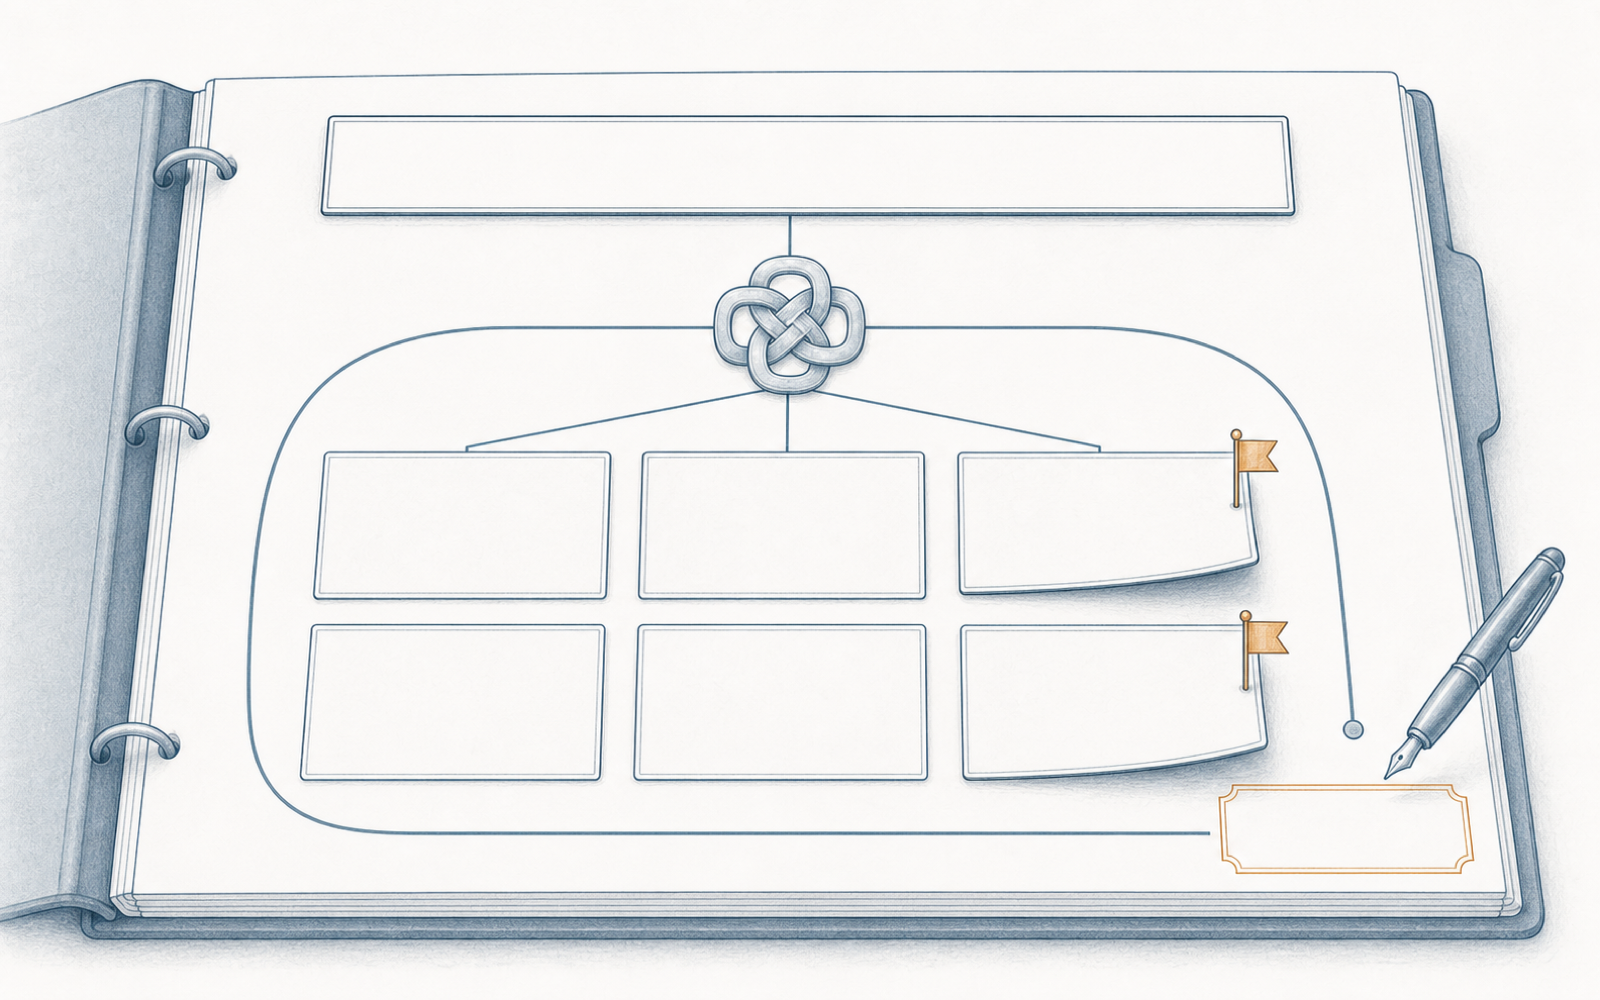
\includegraphics{figures-imagegen/ch20-fig01-live-assurance-case-v01.png}}
\captionof{figure}{活的保证案例会在对象、配置、证据或假设改变时主动暴露过期和重开条件。自动检查负责举旗，最终承担风险的决定和签名仍然属于人。}
\end{minipage}
\end{center}


\begin{noteblock}
\textbf{图后判断}：图中过期标记不等于证据错误，签名框也不表示放行已获授权。本图不替代真实案例的反驳、缺口处置和责任人核验。
\end{noteblock}

\Needspace{6\baselineskip}
\section{RC18：活的安全案例第一次开庭}

正戏其实在开会之前，就已经演完了一半。

升版落地那天，变更获准的消息经由与第 17 章的显式对齐合同送进案例，案例把它翻译
成自己的一条事件，当场举手：三条主张标为过期，论证层七处引用重开，两处经声明
理由保留——保留理由本身也成了对象，第 1 章那句“保留是一个判断，不是一个默认”，
第一次长进了结构里。哪些重开、哪些保留、缺哪张卡，是查询返回的，不是小林熬夜
圈出来的。墙上第二句话——变更影响靠人工圈定——销账。

会前一天，小蔡把案例的状态表调了出来。这一次，六张绿卡的后代第一次自己开口。

\Needspace{8\baselineskip}
问题：此刻 RC18 的案例里，每一路证据各自作证到哪里、状态如何？

\nopagebreak[4]
\begin{codebox}
\begin{Verbatim}[fontsize=\small,breaklines=true,breakanywhere=true,breaksymbolleft={},breaksymbolright={}]
SELECT ?evidence ?testifiesTo ?scope ?status WHERE {
  rel:Case_RC18 rel:citesEvidence ?evidence .   # 案例到证据的汇总边
  ?evidence rel:testifiesTo ?testifiesTo ;
            rel:scopeNote   ?scope ;
            rel:status      ?status .
}
\end{Verbatim}
\end{codebox}

\begin{center}
\begingroup\small
\setlength{\tabcolsep}{4pt}
\begin{tabularx}{\linewidth}{@{}XXXX@{}}
\toprule
证据 & 作证对象 & 射程要点 & 状态 \\
\midrule
概念边界分析·修订版 & RC18 相关项边界 & 选定场景内的危害与目标点名 & 在案 \\
硬件失效率评估 & H3.2 控制器 & 声明剖面与诊断假设之内 & 在案 \\
软件回归·正式构建 & SW1.8.4 加 C41 & 既定测试集与判据之内 & 在案 \\
台架定向补测 & RC18 目标配置 & 边界工况重跑，含低温冷起动 & 在案 \\
冲击振动试验 & 局部机械总成 & 升版不波及，保留理由在案 & 保留 \\
生产写入检查 & RC18 镜像与批次 & 声明工位与批次内写入正确 & 在案 \\
\bottomrule
\end{tabularx}
\endgroup
\end{center}

第 1 章里，这张表是陈工一句一句问出来的；收口评审上，是四个专业、两家单位
两个下午挂出来的；今天它是一条查询。郑工坐在老位置上，第一次不用翻记录念配置——他的台架卡
自己报了家门。开放项也在表外分栏立着，一条不藏：台架异常读数，至今未复现，
状态未知，看守在案；首批现场回传未满一个完整高温季，声明为缺口，窗口另计。
缺口与未知不再靠自觉罗列，它们是案例的常驻对象。

会好像没什么可开的了。老何先把这层意思说了出来：“都绿了，门禁也都过了，那这会
就走个过场呗——签字画押，散会吃饭。”这话在产线上是常识：放行流程电子化这么多
年，绿灯放行天经地义。可它恰好是当年那句“都通过了还等什么”的孙子辈——门禁
通过是机器建立的第三层绿，授权是只有人才能建立的第四层；让绿灯自动生成签字，
等于把残余风险的承担委托给一段没有肩膀的逻辑。反过来也有人劝陈工按老规矩把
三百份文件重读一遍再签——也不必：人重读机器已经核对过的东西，是用勤奋冒充
责任；人该读的是机器压不掉的那几页——未知要不要继续背着走，缺口的窗口给多长，
取舍认不认，代价谁来担。\textbf{机器把案例算到“可签”，人把名字签成“担责”——这两步，谁也替不了谁。}

方工宣读独立评估：建议接受，附条件。他的评估这一次也换了做法——挑战不再是
通读之后的观感，而是一份反向查询清单：他专挑案例声称“已闭合”的分支，逐条查
论证的理由链断不断、引用的证据在不在射程内、冲突处置有没有绕过看守。评估的人
和拿主意的人依旧分开坐，只是挑战者手里第一次有了撬棍。附的条件写成了三条重开：
台架异常读数复现即重开；决定窗口到期即重开；下一轮升版获准即重开——第三条
与当年那条不同：当年钉的是点名的一版，这一次钉住任何下一轮，是变更那次演习
教会所有人的。然后，是助手的最后一个动作。

这段记法在说什么：助手把它能做的最后一件事做成了一个对象——一份提议；决定对象
\Needspace{8\baselineskip}
另立，属于有权角色。两个对象之间那条边，是整个试点最重要的一条边。

\nopagebreak[4]
\begin{codebox}
\begin{Verbatim}[fontsize=\small,breaklines=true,breakanywhere=true,breaksymbolleft={},breaksymbolright={}]
# 最后一步：机器提议，人决定（示意记法）
rel:Proposal_RC18 a rel:AgentProposal ;
    rel:proposes         rel:Decision_RC18 ;
    rel:basedOnCaseState rel:CaseState_AtSigning ;  # 签署时刻的案例状态
    rel:status           rel:ProposedOnly .         # 提议，不是决定
rel:Decision_RC18 a rel:AuthorizationDecision ;
    rel:acceptedBy rel:Role_ReleaseAuthority ;      # 有权角色，今天是陈工
    rel:withReopen rel:Reopen_AnomalyRecur ,
                   rel:Reopen_WindowExpiry ,
                   rel:Reopen_NextUpgrade ;
    rel:scopeNote  "仅授权本轮放行，不授予永久可信" .
\end{Verbatim}
\end{codebox}

陈工签字之前，把桌上的三样东西各按了一下，像老师傅清点工具：案例——大家在谈
什么，一查便知；活动记录——世界上真发生了什么，台架和产线说了算；这支笔——
接下来由谁承担什么，只有他能落。然后他签了。决定对象引用的是签署那一刻的案例
状态：将来任何人回看这个决定，看见的都是陈工当时看见的那份账，不多一页，不少
一页。墙上第三句话——安全案例是死文档——销账：从签字的下一刻起，产线在写入
新的批次，现场在回传新的工况，下一轮升版排上日程，而案例会跟着标注、跟着举手、
跟着把该重开的分支交回人的手上。它活着。

散会时，陈工在白板前站了一会儿。试点开始前写下的那行“RC17，已接受，附条件”
还在。他拿起板擦，把它擦掉了：“记得这件事的，如今不止一块白板。”小唐望着投影
上还亮着的状态表，忽然说：“我现在知道当年那句‘还在等什么’在等什么了——等的
就是这张表，和肯在它下面签名的人。”

会散了，试点结项。可这本书，还欠着三个问题。

\Needspace{6\baselineskip}
\section{谁在指挥，谁在记得，谁有权改写}

先把边界说老实，免得把结项说成神话。这一年建起来的十个本体，没有让 RC18 更安全
一分——安全是台架的补测、产线的校验、设计的余量挣来的，三元组挣不来；本体做到
的，是让“它是否可信”从一句没人能查的口号，变成随时可查、可反驳、也可推翻的
问题。门禁看得住声明过的维度，看不住没人声明的维度：真正的意外，向来从没人想到
要建模的方向进来，所以完备性声明与人的看守永不下岗。十个本体也仍然是十个——
隔壁 ENV-01 的团队来旁听了 RC18 的评审，带走的是问法、结构和纪律，一条业务事实
也没带走，也不该带走；他们的世界，要用他们自己的证据重新回答。

然后，三个问题可以收账了。

谁在指挥？是人。一整年里，助手提议过几千次、执行过几百回，每一次都在门禁与审计
的圈里；它的最后一个动作，是一份状态写着“仅为提议”的对象。指挥从没有换过手。

谁在记得？从前的答案是：加班的人、抽屉，和某位工程师的私人记忆——郑工的差异
说明靠他记得，小林的影响清单靠他记得，深夜的对表靠小蔡恰好没睡。现在的答案是：
一份随产品一起活着的结构在记得，人从记忆的载体，退回记忆的看守与主人。这是
试点真正交付的东西。

谁有权改写这份记忆？还是有权的人——本体没有没收任何人的权力。但从今往后，改写
要留下名字：谁改的、依据什么、经过哪道门禁、谁授权的，全部在案。有权的人仍然
可以改写记忆，却再也不能无痕地改写记忆；而写下每一条的人，会一直留在他写下的
那一行上。

导读的期票，最后兑现一次。合上全书之前，做三件事：翻出你手头最近的安全案例，
找到主张—论证—证据里“论证”那一层，问它上一次产品变更之后动过没有——没动过，
它多半已经死了；抽出放行包里任意两份报告，看有没有“绑定在哪个快照”这一行——
没有这一行，下一个深夜对表的人就还得是你；再找到上一次授权决定，看它引用的是
签署时刻的案例状态，还是一句“以当时材料为准”。三件事做完，你就知道自己离那份
活的案例还有几步。

结项一周后，郑工来找小蔡。他递了退休报告，下个月交台架。两个人一起做的最后
一件事，是移交那条重开条件的看守：屏幕上，看守角色的占位从他换成他带了三年的
年轻人。系统请郑工本人确认移交——哪怕是离开，放下看守也是一个只有他有权作的
决定。他按了确认，然后盯着那个条目看了很久。看守人一栏换了名字；第一行没有
换——那里仍然记着，当年是谁把那页读数从抽屉里拿出来，放到了所有人看得见的
地方。

“我以前最怕的，”郑工说，“是我走了，这一页跟着我走。现在它留下了，名字也留下
了。够了。”

小蔡送他到楼下。电梯门合上之前，郑工朝她挥了挥手。她回到工位，那条重开条件
安安静静地亮在屏幕上：看守换了人，写下它的人继续被看见。

一件产品值得被相信，从来不是因为谁说了一句“放心”——而是因为有一群人，肯把
自己的名字一行一行留在它活着的记忆里。


\begin{noteblock}
\textbf{本章注记}：本章的试点情节、人物、事故经过与全部产品数字（候选代号、软硬件与
标定版本、时间跨度、台数等）均为合成教学材料，不对应任何真实企业、真实产品或
真实个人。正文中的片段为教学示意，不构成完整形式化定义；唯一可执行版本是
\nolinkurl{semantica.chapter_packages.vol2.ch20}，当前为 \nolinkurl{partial}、release \nolinkurl{blocked}。
本章对安全案例与发布保证活动的转述为自然语言概括，
精确要求以标准原文为准；本章不构成对任何实际系统的判定或放行结论。
\end{noteblock}
